\section{Desarrollo basado en MLOps}
    MLOps (Machine Learning Operations) es una extensión de la metodología DevOps (Development Operations)
    que se enfoca en la integración, desarrollo y gestión del software de la mano del ciclo de vida del modelo.
    Los pilares fundamentales se basan en la automatización y la mejora progresiva de la calidad del modelo, 
    lo que permite una implementación y puesta en producción mucho más efectiva. Para lograrlo, utiliza herramientas 
    y técnicas que permiten monitorizar, testear, mejorar y adaptar no solo los modelos sino toda la arquitectura
    del sistema de forma continua y escalable. Aquí podemos observar el flujo de información dentro de una 
    arquitectura MLOps. 

    \begin{figure}[ht]
        \centering
        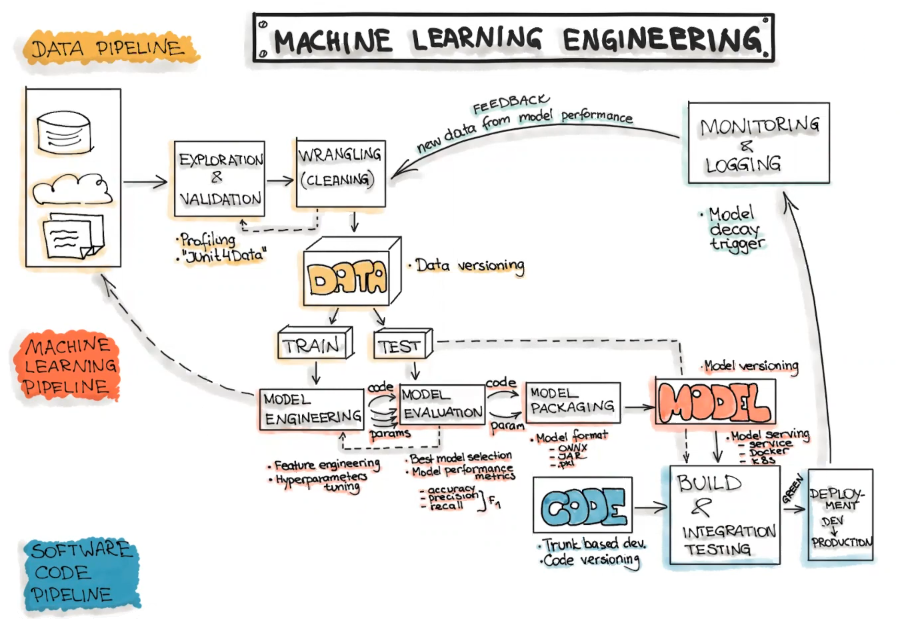
\includegraphics[scale=0.55]{architecture.png}
        \caption{Arquitectura MLOps}
        \label{fig:architecure-mlops}
    \end{figure}

    \subsection{Principios de MLOps}
    A continuación, vamos a detallar los principios de MLOps que vamos a seguir en el desarrollo de nuestro proyecto.
    En esta sección se incluyen los puntos más importantes de la metodología, durante todo el desarrollo intentaremos
    cumplir con ellos en la medida de lo posible, ya que pueden darse situaciones en las que sea totalmente imposible
    satisfacerlos al completo.

    \begin{itemize}
        \item \textbf{Automatización}: la automatización es la clave para la eficiencia y la escalabilidad.
        Aqui incluimos tareas como la generación de datos, el despliegue del modelo, la evaluación y 
        la puesta en producción.
        \item \textbf{Testeo}: garantiza que tanto la funcionalidad como el desempeño del modelo están evaluados correctamente. 
        Esencial en Machine Learning para identificar problemas y mejorar la confianza en los resultados.
        \item \textbf{Versionado}: es importante tener un control de versiones de los datos, el código y los modelos. 
        Puede variar el método dependiendo de la herramienta que se utilice, pero existen estándares como Git para la gestión
        de código y GitHub/GitLab para el almacenamiento de los repositorios.
        \item \textbf{Reproducibilidad}: es necesario poder reproducir los resultados de forma consistente, puede ser
        complicado en Machine Learning debido a la naturaleza aleatoria de los algoritmos. Igualmente aquí se trataran
        las herramientas y medidas necesarias para lograrlo.
        \item \textbf{Monitorización}: es importante tener un control de los modelos en proceso de entrenamiento o de producción.
        Por ello, recolectar estadisiticas en tiempo de procesamiento nos ayudará a generar nuevas hipotesis para las proximas interaciones. 
    \end{itemize}

    \subsection{Metodología de trabajo}
    Una de las características de los proyectos de Machine Learning es que son tecnologías en constante evolución, el 
    desarrollo no es un proceso sencillo y requiere de un enfoque coordinado por parte de los diferentes
    equipos que lo conforman para asegurar su sostenibilidad a largo plazo. Es fundamental poder adapatarse a los cambios
    de forma agil, sin que esto suponga un deterioro del nivel de productividad o que ralentice el avance de nuevas
    funcionalidades.\medskip 

    Podemos identificar tres fases principales: diseño, desarrollo del modelo y operaciones. Cada fase tiene un enfoque
    específico y requiere una serie de tareas para garantizar el éxito del proyecto. La fase de diseño, 
    se definen los objetivos y requisitos del proyecto, se identifican los datos necesarios para el entrenamiento y 
    se establecen los criterios de éxito. La fase de desarrollo del modelo, se preparan los datos, se entrena el modelo 
    y se evalúa su rendimiento. También se realiza la validación y se toman las decisiones sobre el modelo final a utilizar. 
    Finalmente, en la fase de operaciones, se integra el modelo en la infraestructura existente, se monitorea su rendimiento
    y se extraen conclusiones para futuras iteraciones. Al repartir las responsabilidades en diferentes fases, aislamos los erroes junto con la carga de trabajo y podemos avanzar 
    sin la preocuapacion de que un bug o un cambio requisitos afecte al resto del equipo. 
    
    \begin{figure}[ht]
        \centering
        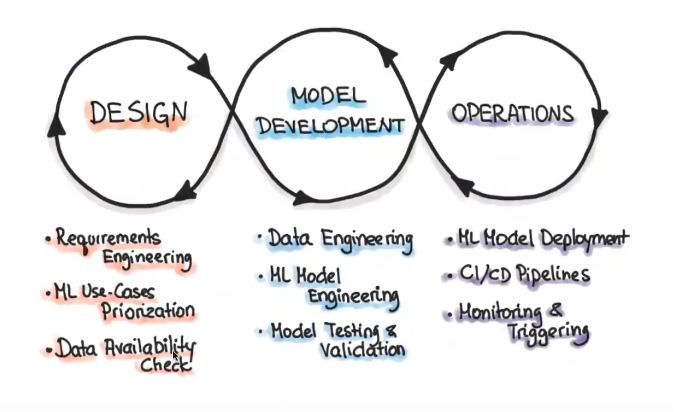
\includegraphics[scale=0.5]{proceso-mlops.png}
        \caption{Metodología MLOps}
        \label{fig:proces-mlops}
    \end{figure}

    Para visualizar de forma más clara la ventaja que supone este enfoque frente a uno tradicional, a continuación 
    se mencionara un ejemplos de una posible situacion real. \textbf{Ejemplo:} Tenemos un modelo que actualmente está alojado en AWS y queremos migrarlo a Azure, debido a que
    utilizamos MLOps existe configurada una action que en el momento que el equipo publica una nueva release
    automáticamente despliega el modelo en el servidor cloud. La parte del equipo encargada de las operaciones procede
    a configurar el nuevo servicio y modificar la action para redirigir el despliegue al nuevo servidor. Durante este
    tiempo, el equipo de desarrollo a podido avanzar en nuevas mejoras para el modelo y ahora se disponen a volver
    a publicar los cambios. Ellos no han notado ningún cambio, pero a nivel de infraestructura se ha realizado una 
    completa migracion sin afectar en ningún momento en el desarrollo.


\pagebreak